\documentclass{standalone}

\usepackage{tikz}
\usetikzlibrary{shapes.geometric}
\usetikzlibrary{math}
\usetikzlibrary{decorations.text}
\usepackage{import}

\import{../../}{wellington-commands}

\begin{document}

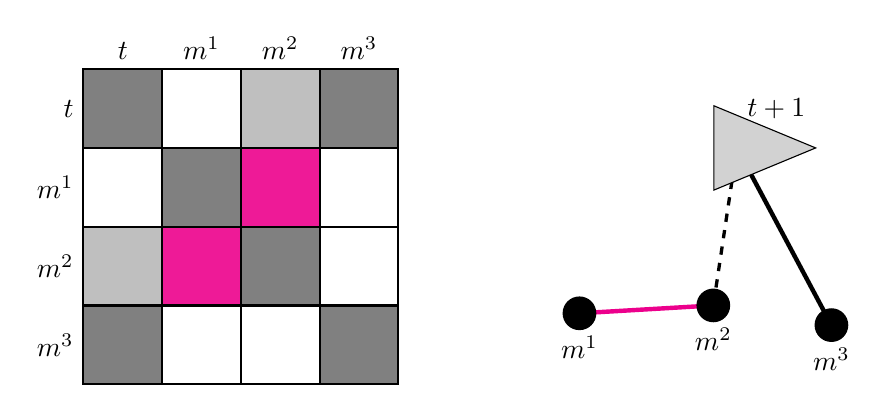
\begin{tikzpicture}
  \tikzmath{
    \m = 4;
    \rx = 0;
    \ry = \m-1;
    coordinate \landmark, \robotpos, \oldrobotpos;
    \oldrobotpos = (6.5, \m-1);
    \robotpos = (8.3, \m-1);
    \landmark1 = (\m+2.3, 0.9);
    \landmark2 = (\m+4, 1);
    \landmark3 = (\m+5.5, .75);
  };
  \def\activeLandmarks{\landmark1, \landmark2, \landmark3}
  \def\passiveLandmarks{}

  % matrix 
  \draw [step=1.0,black, thick] (0, 0) grid (\m, \m); 

  % % labels
  % % % robot
  \path (\rx, \ry) -- (\rx, \ry+1) node [midway, anchor=east] {$\robotstate{t}$};
  \path (\rx, \ry+1) -- (\rx+1, \ry+1) node [midway, anchor=south] {$\robotstate{t}$};

  % % % mapa
  \tikzmath{
    int \i;
    for \i in {1,...,3}{
      {
        \path (\i, \m) -- (\i+1, \m) node [midway, anchor=south] {$\bvec{m}^\i$};
        \path (0, \m-\i) -- (0, \m-\i-1) node [midway, anchor=east] {$\bvec{m}^\i$};
      };
    };
  };

  % % draw active
  \filldraw[fill=gray, thick] (\rx, \ry) rectangle ++(1,1);
  \tikzmath{
    for \i in {1, 2, 3}{
      if \i != 1 then{
        if \i == 3 then{
          {
            \filldraw[fill=gray, thick] (\rx+\i, \ry) rectangle ++(1,1);
          };
        }else{
          {
            \filldraw[fill=lightgray, thick] (\rx+\i, \ry) rectangle ++(1,1);
          };
        };
      };
                {
        \filldraw[fill=gray, thick] (\i, \m-\i-1) rectangle ++(1,1);
      };
      if \i != 1 then{
        if \i == 3 then{
          {
            \filldraw[fill=gray, thick] (0, \m-\i-1) rectangle ++(1,1);
          };
        }else{
          {
            \filldraw[fill=lightgray, thick] (0, \m-\i-1) rectangle ++(1,1);
          };
        };
      };
    };
  };
  % % draw correlation by motion
  \tikzmath{
    for \i in {1,2}{
      for \j in {1,2}{
        if \i != \j then{
          {
            \filldraw[fill=magenta!90, thick] (\j, \m-\i-1) rectangle ++(1,1);
          };
        };
      };
    };
  };
  %
  
  % landmarks
  % % active landmarks
    % links
    \draw [very thick, dashed] (\robotpos) -- (\landmark2) node[midway] (L_2) {};
    \path [] (\robotpos) -- (\landmark1) node[midway] (L_1) {};
    \draw [ultra thick] (\robotpos) -- (\landmark3) node[midway] (L_3) {};
    \foreach \activeLandmark[count=\i] in {\landmark1, \landmark2} {
      \foreach \pos[count=\j] in {\landmark1, \landmark2}{
        \ifnum \i<\j
          \draw [ultra thick, magenta] (\activeLandmark) -- (\pos) node[midway] (L_\i_\j) {};
        \fi
      }
    }

    \foreach \activeLandmark in \activeLandmarks {
      \filldraw [fill=black, thick, draw=black] (\activeLandmark) circle (.2);
    }
  
    % % not active landmarks
    \foreach \passiveLandmark in \passiveLandmarks{
      \filldraw [fill=white, thick, draw=black] (\passiveLandmark) circle (.2);
    }

    % % labels
    \foreach \pos [count=\i] in {\landmark1, \landmark2, \landmark3}{
      \node[anchor=north, label={[yshift=-0.7cm]$\bvec{m}^\i$}] at (\pos) {};
    }
  %
  
  % robot 
  % % body
  \node[isosceles triangle,
    draw,
    fill=gray!35,
    scale=2.5] (T)at (\robotpos){};
  
  % % label
  \node (RL)at(\robotposx+.5cm, \m-0.5) {$\robotstate{t+1}$};
  %

\end{tikzpicture}
\end{document}